\chapter{The Expanding Newtonian Universe}

\lectureoverview{Modern cosmology begins when the universe itself is treated as a physical system. Starting from large-scale isotropy and homogeneity, we introduce a comoving grid and encode its motion in a single scale factor \(a(t)\). Newton's shell theorem then turns the gravitational many-body problem into an equation for \(a(t)\). Energy conservation distinguishes recollapsing, critical, and eternally expanding universes, and the critical matter-dominated case gives the first Friedmann equation and the law \(a(t)\propto t^{2/3}\).}

\section{When Cosmology Became Physics}

Cosmology is ancient as a subject, but quantitative cosmology is young. For the present purpose there is no need to begin with the Greeks. The useful historical starting points are Hubble's discovery of cosmic expansion in the second quarter of the twentieth century and, later, the recognition of the roughly three-kelvin microwave background as a remnant of a hot early universe.

Before measurements became precise, much of astronomy necessarily resembled natural history. One found an unusual star, classified a peculiar galaxy, measured what could be measured, and assembled a catalogue of objects. Those objects were certainly physical systems: they carried angular momentum, contained chemical elements, and obeyed mechanics. The decisive change was to treat the \emph{whole universe} as one physical system, governed by equations accurate enough to confront observation.

That is the subject here. We shall not merely list the contents of the universe; we shall ask for its variables, its motion, and its dynamical law. Equations are not an ornament added after the cosmology. They are the means by which the universe becomes a physics problem.

Historically, the expanding universe was understood in the language of general relativity. Logically, however, much of the first argument is Newtonian. A seventeenth-century physicist who had guessed the right large-scale motion could have derived a remarkably good model. The point of beginning with Newton is not to replace relativity, but to expose the mechanics that relativity later reorganizes geometrically.

\section{Isotropy, Homogeneity, and the Cosmological Principle}

The first step is observational. On sufficiently large scales the universe is approximately \emph{isotropic}: after averaging over patches of sky and looking beyond the foreground of the Milky Way, it looks much the same in every direction. This is not a statement of exact uniformity. Looking directly at a nearby star is different from looking into an empty patch, and the distribution of matter contains real structure. Isotropy is an averaged large-scale statement.

Homogeneity is a different statement. It says that the averaged universe is the same from place to place. An observer many galaxies away should see, after the same large-scale averaging, approximately the same kind of universe that we see.

For the first approximation, a galaxy may be treated simply as a mass point. The visible universe contains roughly
\begin{equation}
N_{\rm gal}\sim 10^{11}
\end{equation}
galaxies, each with of order \(10^{11}\) stars. This gives approximately \(10^{22}\) stars. If one uses ten planets per star as a deliberately rough order-of-magnitude estimate, one arrives at \(10^{23}\) planets, amusingly close to a mole of planets. The numerical estimate is not part of the dynamics, but it fixes the scale of the system being idealized.

\begin{classroomqa}
\classquestion{How many galaxies are there within the observable universe, to order of magnitude?}
\lecturerresponse{About one hundred billion, or \(10^{11}\). With roughly \(10^{11}\) stars per galaxy, that means approximately \(10^{22}\) stars in the visible universe. These are useful scale estimates to keep in mind even though the calculation below replaces each galaxy by a single mass point. \lecturetimestamp{00:06:08--00:07:05}}
\end{classroomqa}

Why should isotropy around us suggest homogeneity? Imagine an isotropic distribution that is \emph{not} homogeneous. Its density would have to vary with distance from us while remaining independent of direction: in effect, it would form a pattern of concentric shells about our position. An observer displaced from the common center would no longer see isotropy. Thus there are two possibilities:
\begin{enumerate}
\item we occupy a distinguished center about which the universe has been arranged; or
\item the large-scale distribution is approximately homogeneous, so no occupied point is distinguished.
\end{enumerate}
The second possibility is the economical one. Isotropy, together with the refusal to assign ourselves a privileged cosmic position, leads to homogeneity.

\begin{classroomqa}
\classquestion{What form could an isotropic but inhomogeneous distribution take?}
\lecturerresponse{Its variation could depend only on distance from us, producing a shell-like pattern centered on our position. Move the observer away from that center and the pattern ceases to be isotropic. Unless our location is special, isotropy therefore points to homogeneity. \lecturetimestamp{00:07:06--00:08:54}}
\end{classroomqa}

The combined assumption is called the \emph{cosmological principle}: on sufficiently large scales, the universe is spatially homogeneous and isotropic. Calling it a principle does not prove it. Historically, cosmologists adopted the assumption before observations justified it strongly. Its standing comes from empirical success.

Nor is homogeneity exact. Galaxies form clusters and superclusters, and there have long been discussions of structures extending across very large fractions of the visible sky. The appropriate claim is that fluctuations average away when the averaging region is sufficiently large---of order hundreds of millions to roughly a billion light-years in this introductory discussion. The scale may be refined by observation; the method is to coarse-grain until local structure no longer dominates the description.

\begin{classroomqa}
\audiencequestion{Does the uniformity of the cosmic microwave background provide evidence for the cosmological principle?}
\lecturerresponse{Yes. The cosmological principle was proposed before there was strong observational warrant for it, but the microwave background later showed that the primordial universe was extraordinarily smooth. Galaxies and clusters grew from small departures from that smooth state; they do not erase the large-scale evidence for it. \lecturetimestamp{00:10:53--00:11:43}}
\end{classroomqa}

\section{A Grid That Moves with the Galaxies}

Once the observational approximation is chosen, we must choose variables. One classroom answer to the question "What is the first step in formulating a physics problem?" is to know the variables; the traditional answer is to sharpen one's pencil. Here the important variable is found by choosing coordinates well.

Imagine a three-dimensional grid carrying labels \(x,y,z\). These labels need not be distances measured in meters. They are coordinate numbers. Choose the grid so that, after small peculiar motions have been averaged away, every galaxy remains at a fixed grid point. The galaxies are then \emph{comoving}.

Such a choice would be useless if galaxies moved randomly. Observation instead reveals a coherent large-scale motion. Neighboring grid cells may expand or contract, but the same expansion or contraction occurs everywhere. All physical distances can therefore be written as a common time-dependent scale multiplied by a fixed coordinate separation.

For two galaxies \(A\) and \(B\),
\begin{equation}
d_{AB}(t)=a(t)\sqrt{(x_A-x_B)^2+(y_A-y_B)^2+(z_A-z_B)^2}.
\label{eq:c01-physical-distance}
\end{equation}
If they differ only in the \(x\)-coordinate, this reduces to
\begin{equation}
d_{AB}(t)=a(t)\,\Delta x_{AB}.
\end{equation}
The function \(a(t)\) is the \emph{scale factor}. Its absolute normalization is conventional: multiplying all comoving coordinates by a constant and dividing \(a\) by the same constant changes no physical distance. Ratios such as \(a(t_2)/a(t_1)\), and derivatives divided by \(a\), carry the physical information.

Differentiate equation~\eqref{eq:c01-physical-distance}. The comoving separation is fixed, so
\begin{equation}
v_{AB}=\dot a\sqrt{(\Delta x)^2+(\Delta y)^2+(\Delta z)^2}.
\end{equation}
Dividing by the physical distance gives
\begin{equation}
\frac{v_{AB}}{d_{AB}}=\frac{\dot a}{a}\equiv H(t),
\label{eq:c01-hubble-parameter}
\end{equation}
or
\begin{equation}
\boxed{v_{AB}=H(t)d_{AB}.}
\label{eq:c01-hubble-law}
\end{equation}
This is Hubble's law in the ideal homogeneous flow.

The name "Hubble constant" can mislead. At one cosmic time the same value of \(H\) applies at every place in the homogeneous model, but \(H(t)\) generally changes with time. Spatial universality is not temporal constancy.

\begin{classroomqa}
\audiencequestion{By writing every distance as one common \(a(t)\) times a fixed coordinate separation, have we already assumed Hubble's law?}
\lecturerresponse{The ansatz is certainly motivated by Hubble's observation; it would not be guessed without evidence for coherent recession. Its value is to organize that evidence. Instead of assigning an independent velocity to every galaxy, one describes a single expanding grid. Once that description is adopted, the proportionality \(v=Hd\) follows by differentiation. \lecturetimestamp{00:24:20--00:25:33}}
\end{classroomqa}

The same motion admits two verbal descriptions. One may say that galaxies move apart through space, or that galaxies remain at fixed comoving positions while the grid---and hence physical space between them---expands. At this stage these are two coordinate descriptions of the same mathematics. General relativity will make the expanding-space language especially natural, but no observation can distinguish two descriptions that assign the same physical separations at every time.

\section{Mass Bookkeeping in a Comoving Cell}

Before introducing gravity, keep track of mass. Consider a small coordinate cell with coordinate volume
\begin{equation}
\Delta V_{\rm com}=\Delta x\,\Delta y\,\Delta z.
\end{equation}
It must still be large enough to contain many galaxies, so that local fluctuations may be averaged. Let \(\nu\) denote mass per unit comoving coordinate volume. The mass in the cell is
\begin{equation}
\Delta M=\nu\,\Delta x\,\Delta y\,\Delta z.
\label{eq:c01-comoving-mass}
\end{equation}
Because the cell moves with the matter, no galaxy crosses its boundary in the ideal flow, and \(\Delta M\) is constant.

Each physical edge is longer than its coordinate edge by a factor \(a(t)\). The physical volume is therefore
\begin{equation}
\Delta V_{\rm phys}=a^3(t)\,\Delta x\,\Delta y\,\Delta z.
\end{equation}
The physical mass density is
\begin{equation}
\boxed{\rho(t)=\frac{\Delta M}{\Delta V_{\rm phys}}=\frac{\nu}{a^3(t)}.}
\label{eq:c01-density-dilution}
\end{equation}
Expansion dilutes pressureless matter as \(a^{-3}\); contraction concentrates it by the same law.

Up to this point nothing dynamical has been assumed. We have used Euclidean geometry, a kinematic ansatz, and conservation of mass in a comoving cell. Now gravity enters.

\section{Now Enters Newton}

A tempting but incorrect picture says that an infinite uniform distribution of matter should remain static because the pull from one side is canceled by the pull from the other. The flaw is that this informal cancellation does not supply a consistent equation for relative acceleration. Newton's shell theorem gives the correct organization of the force.

Choose any galaxy as an origin \(O\), and consider a galaxy \(A\) at fixed comoving radius
\begin{equation}
R=\sqrt{x^2+y^2+z^2}.
\end{equation}
Its physical radius, radial velocity, and radial acceleration are
\begin{equation}
d=aR,
\qquad
\dot d=\dot a R,
\qquad
\ddot d=\ddot a R.
\label{eq:c01-radial-kinematics}
\end{equation}

\begin{figure}[ht]
\centering
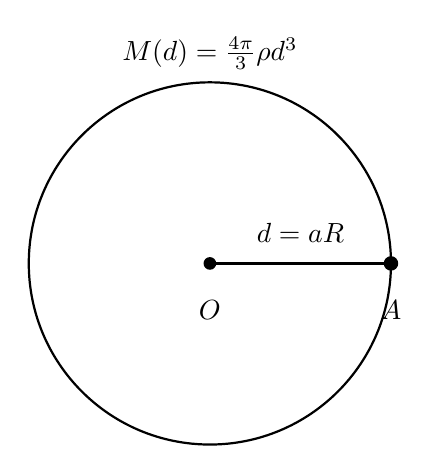
\begin{tikzpicture}[scale=1.15]
\draw[thick] (0,0) circle (2);
\fill (0,0) circle (0.07);
\fill (2,0) circle (0.08);
\draw[thick] (0,0) -- (2,0);
\draw (1,0.12) node[above] {\(d=aR\)};
\draw (0,-0.3) node[below] {\(O\)};
\draw (2,-0.3) node[below] {\(A\)};
\draw (0,2.32) node {\(M(d)=\frac{4\pi}{3}\rho d^3\)};
\end{tikzpicture}
\caption{The Newtonian reduction. For the acceleration of galaxy \(A\), the exterior shells cancel and the mass inside radius \(d\) acts as though concentrated at \(O\).}
\label{fig:c01-newton-sphere}
\end{figure}

For a spherically symmetric mass distribution, the net force from matter outside the sphere through \(A\) vanishes. The matter inside acts as though it were concentrated at the center. The enclosed mass is
\begin{equation}
M(d)=\frac{4\pi}{3}\rho d^3.
\label{eq:c01-enclosed-mass}
\end{equation}
Newton's inverse-square law then gives the acceleration of \(A\):
\begin{equation}
\ddot d=-\frac{GM(d)}{d^2}.
\end{equation}
Using equation~\eqref{eq:c01-radial-kinematics},
\begin{align}
\ddot a R
&=-\frac{G}{d^2}\left(\frac{4\pi}{3}\rho d^3\right) \\
&=-\frac{4\pi G}{3}\rho d \\
&=-\frac{4\pi G}{3}\rho aR.
\end{align}
The comoving radius cancels, leaving
\begin{equation}
\boxed{\frac{\ddot a}{a}=-\frac{4\pi G}{3}\rho.}
\label{eq:c01-acceleration}
\end{equation}
This cancellation is the consistency test. Every comoving galaxy, regardless of \(R\), obeys the same equation for the same scale factor.

Substituting equation~\eqref{eq:c01-density-dilution} gives either of the equivalent forms
\begin{equation}
\frac{\ddot a}{a}=-\frac{4\pi G\nu}{3a^3},
\qquad
\ddot a=-\frac{4\pi G\nu}{3a^2}.
\label{eq:c01-acceleration-nu}
\end{equation}
The first form displays fractional acceleration; the second isolates \(\ddot a\). Keeping \(a\) on the left is a convention, not a change of physics.

\begin{classroomqa}
\audiencequestion{The origin was arbitrary, yet every force in the calculation points toward it. How can a different choice of origin give the same universe?}
\lecturerresponse{The equation concerns relative motion. Repeating the calculation around any other galaxy gives the same equation because homogeneity makes the enclosed mass depend only on physical radius. If one transforms to an accelerating frame attached to another galaxy while retaining forces referred to the first origin, the corresponding inertial force must also be included. Choosing a central rest frame merely avoids carrying that extra bookkeeping. The invariant result is equation~\eqref{eq:c01-acceleration}, not a distinguished center. \lecturetimestamp{00:43:56--00:46:58}}
\end{classroomqa}

\begin{classroomqa}
\audiencequestion{Would the result survive if the comoving mass density \(\nu\) varied from place to place?}
\lecturerresponse{Not in this one-function form. The clean cancellation depends on \(M\propto d^3\) with the same proportionality everywhere. If \(\nu\) varied appreciably across the averaging scale, different regions would require different local dynamics and a single homogeneous scale factor would no longer describe them. Homogeneity is doing essential work. \lecturetimestamp{00:47:05--00:47:51}}
\end{classroomqa}

\begin{classroomqa}
\audiencequestion{Why write \(\ddot a/a\) rather than move the factor \(a\) to the right?}
\lecturerresponse{Either form is correct. Cosmology conventionally writes the fractional acceleration \(\ddot a/a\), partly because it can be compared directly with the fractional expansion rate \(H=\dot a/a\). Multiplying through by \(a\) gives the identical differential equation. \lecturetimestamp{00:50:36--00:51:29}}
\end{classroomqa}

Equation~\eqref{eq:c01-acceleration} immediately rules out a static homogeneous Newtonian universe filled with ordinary matter. A static scale factor would have \(\ddot a=0\), whereas positive density makes the right-hand side negative. This does \emph{not} yet tell us whether the universe is expanding or contracting. It tells us only the sign of the acceleration.

\section{Negative Acceleration Is Not Contraction}

The distinction between velocity and acceleration is elementary but decisive. A Ferrari moving forward on the Autobahn can have positive velocity while braking with negative acceleration. Likewise, a universe can have
\begin{equation}
\dot a>0,
\qquad
\ddot a<0:
\end{equation}
it is expanding, but the expansion is slowing.

To decide whether the motion eventually reverses, compare the cosmological problem with a test particle moving radially in the gravitational field of the Earth. Let \(x\) now denote the particle's physical distance from a central mass \(M\); it is unrelated to the earlier comoving coordinate. Newton's equation is
\begin{equation}
\ddot x=-\frac{GM}{x^2}.
\label{eq:c01-particle-force}
\end{equation}
The acceleration always points inward. A particle thrown outward may nevertheless continue outward for a long time, or forever. A particle already moving inward acquires an increasingly negative velocity. The force law alone does not decide which motion occurs; initial conditions do.

\begin{classroomqa}
\audiencequestion{Does \(\ddot a<0\) mean that the universe is contracting?}
\lecturerresponse{No. Contraction means \(\dot a<0\). Negative \(\ddot a\) means only that \(\dot a\) decreases with time. If \(\dot a\) begins positive, gravity slows the expansion; whether it reaches zero depends on the initial expansion speed, exactly as the fate of an outward-moving projectile depends on whether it is below or above escape velocity. \lecturetimestamp{00:51:30--00:56:18}}
\end{classroomqa}

\begin{figure}[ht]
\centering
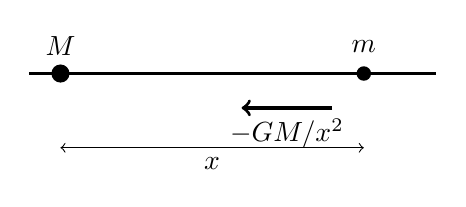
\begin{tikzpicture}[scale=1.15]
\fill (0,0) circle (0.1);
\draw (0,0.3) node {\(M\)};
\draw[thick] (-0.35,0) -- (4.15,0);
\fill (3.35,0) circle (0.08);
\draw (3.35,0.3) node {\(m\)};
\draw[->,very thick] (3.0,-0.38) -- (2.0,-0.38)
  node[midway,below] {\(-GM/x^2\)};
\draw[<->] (0,-0.82) -- (3.35,-0.82)
  node[midway,below] {\(x\)};
\end{tikzpicture}
\caption{The radial one-particle problem used to separate the sign of acceleration from the direction and fate of motion.}
\label{fig:c01-particle-sketch}
\end{figure}

Energy makes the alternatives transparent. The conserved mechanical energy is
\begin{equation}
E=\frac12 m\dot x^{\,2}-\frac{GMm}{x}.
\label{eq:c01-particle-energy}
\end{equation}
The potential energy is proportional to \(1/x\), not \(1/x^2\); differentiating \(-GMm/x\) produces the inverse-square force.

\begin{figure}[ht]
\centering

\includegraphics[width=0.82\textwidth]{lecture_01_figure_02.png}
\caption{The board at the beginning of the energy argument: a moving test mass and its kinetic term, just before the gravitational potential energy is restored.}
\lectureframe{00:58:57}
\end{figure}

If \(E<0\), an outward-moving particle cannot reach infinity, where its potential energy tends to zero and its kinetic energy is nonnegative. It must stop at finite \(x\) and return. If \(E>0\), it cannot stop, because at a turning point the kinetic energy would vanish and the remaining potential energy would be negative, contradicting conservation of a positive \(E\). The boundary is
\begin{equation}
E=0,
\end{equation}
which defines escape velocity:
\begin{equation}
\frac12 m v_{\rm esc}^2-\frac{GMm}{x}=0,
\qquad
\boxed{v_{\rm esc}^2=\frac{2GM}{x}.}
\label{eq:c01-escape-velocity}
\end{equation}

\begin{figure}[ht]
\centering

\includegraphics[width=0.88\textwidth]{lecture_01_figure_03.png}
\caption{The zero-energy boundary taking shape on the board. The earlier cosmological acceleration equations remain boxed at left while the radial escape problem is developed at right.}
\lectureframe{01:01:37}
\end{figure}

Exactly at escape velocity the particle slows indefinitely. Its speed tends to zero only as \(x\to\infty\); it never reaches a finite turning point. This edge case will be the simplest cosmological model.

\section{The Cosmological Energy Equation}

Return to a galaxy at fixed comoving radius \(R\). By the shell theorem its radial motion is identical to that of a particle moving outside a point mass equal to the mass enclosed by its comoving sphere.

\begin{figure}[ht]
\centering

\includegraphics[width=0.82\textwidth]{lecture_01_figure_04.png}
\caption{The inverse-square force and radial-particle sketch used when the one-particle energy argument is transferred back to cosmology.}
\lectureframe{01:04:14}
\end{figure}

The enclosed mass does not increase as the physical sphere expands. The sphere is comoving, so it always contains the same galaxies:
\begin{align}
M
&=\frac{4\pi}{3}\rho(aR)^3 \\
&=\frac{4\pi}{3}\frac{\nu}{a^3}a^3R^3 \\
&=\frac{4\pi}{3}\nu R^3.
\label{eq:c01-fixed-enclosed-mass}
\end{align}
The first expression appears time dependent only until density dilution is included. The factors of \(a^3\) cancel.

\begin{classroomqa}
\audiencequestion{As the sphere expands, does it enclose more mass?}
\lecturerresponse{No. Its physical radius grows, but its comoving boundary moves with the galaxies. No matter crosses that boundary in the ideal homogeneous flow, and equation~\eqref{eq:c01-fixed-enclosed-mass} shows the cancellation explicitly. \lecturetimestamp{01:04:37--01:05:20}}
\end{classroomqa}

The galaxy's physical speed is \(\dot d=\dot a R\), and its distance from the chosen origin is \(d=aR\). Its conserved Newtonian energy is therefore
\begin{equation}
\boxed{
E=\frac12 m\dot a^{\,2}R^2-\frac{GMm}{aR}.
}
\label{eq:c01-cosmological-energy}
\end{equation}

\begin{figure}[ht]
\centering

\includegraphics[width=0.82\textwidth]{lecture_01_figure_05.png}
\caption{The cosmological kinetic and potential terms on the board. The complete denominator \(aR\) in equation~\eqref{eq:c01-cosmological-energy} follows from the physical radius and the accompanying derivation.}
\lectureframe{01:06:12}
\end{figure}

The three particle-energy cases become three cosmological cases:
\begin{description}[style=nextline]
\item[\(E<0\):] the initial expansion is below escape velocity; \(a(t)\) reaches a maximum and the universe recollapses.
\item[\(E=0\):] the universe is exactly critical; expansion slows forever and approaches zero speed only asymptotically.
\item[\(E>0\):] the initial expansion is above escape velocity; the universe expands forever with nonzero asymptotic recession speed in the Newtonian model.
\end{description}

We begin with the edge \(E=0\). Setting equation~\eqref{eq:c01-cosmological-energy} to zero, canceling \(m\), and dividing by \(a^2R^2/2\) gives
\begin{align}
\frac12\dot a^{\,2}R^2&=\frac{GM}{aR}, \\
\left(\frac{\dot a}{a}\right)^2&=\frac{2GM}{a^3R^3}.
\label{eq:c01-energy-intermediate}
\end{align}
Since
\begin{equation}
\rho=\frac{M}{(4\pi/3)a^3R^3},
\end{equation}
equation~\eqref{eq:c01-energy-intermediate} becomes
\begin{equation}
\boxed{
H^2=\left(\frac{\dot a}{a}\right)^2=\frac{8\pi G}{3}\rho.
}
\label{eq:c01-first-friedmann}
\end{equation}
This is the first Friedmann equation for a spatially flat, matter-only universe with zero cosmological constant, obtained here from Newtonian energy conservation.

\begin{classroomqa}
\classquestion{What happens to a particle launched at exactly escape velocity?}
\lecturerresponse{It slows without ever reversing. Its speed approaches zero only at infinite distance. The zero-energy universe behaves in the same way: \(H\) decreases, but \(\dot a\) remains positive and no finite-time turnaround occurs. \lecturetimestamp{01:10:45--01:12:10}}
\end{classroomqa}

The factors \(4\pi/3\) and \(8\pi G/3\) are not arbitrary decoration. The \(4\pi/3\) is the volume of a sphere, and the factor of two comes from kinetic energy. In general relativity the same \(8\pi G\) appears in Einstein's field equation, and its time-time component leads to the relativistic Friedmann equation. That agreement is not accidental, but the present derivation does not yet include pressure, spatial curvature as geometry, or a cosmological constant.

\section{The Critical Matter-Dominated Solution}

Use the density law \(\rho=\nu/a^3\) in equation~\eqref{eq:c01-first-friedmann}:
\begin{equation}
\left(\frac{\dot a}{a}\right)^2=\frac{8\pi G\nu}{3a^3}.
\label{eq:c01-matter-friedmann}
\end{equation}
The constant \(\nu\) depends on the arbitrary normalization of comoving coordinates. To expose the time dependence, define
\begin{equation}
K\equiv\frac{8\pi G\nu}{3}>0.
\end{equation}
Then
\begin{equation}
\dot a^{\,2}=\frac{K}{a}.
\label{eq:c01-normalized-friedmann}
\end{equation}

\begin{figure}[ht]
\centering

\includegraphics[width=0.76\textwidth]{lecture_01_figure_06.png}
\caption{The matter-dominated Friedmann scaling on the board, first with its constants and then with the essential inverse power of the scale factor exposed.}
\lectureframe{01:14:44}
\end{figure}

The right-hand side of equation~\eqref{eq:c01-normalized-friedmann} is positive at every finite positive \(a\). A turnaround would require \(\dot a=0\), so the critical universe never turns around. Its expansion grows steadily more tired, but never tired enough to stop.

Now solve the equation. One may separate variables directly,
\begin{equation}
a^{1/2}\,da=\sqrt{K}\,dt,
\end{equation}
or follow the lecture and try a power law,
\begin{equation}
a(t)=Ct^p.
\label{eq:c01-power-trial}
\end{equation}
Then
\begin{equation}
\frac{\dot a}{a}=\frac{p}{t},
\qquad
\frac{K}{a^3}=\frac{K}{C^3t^{3p}}.
\end{equation}
Substitution into equation~\eqref{eq:c01-matter-friedmann} gives
\begin{equation}
\frac{p^2}{t^2}=\frac{K}{C^3t^{3p}}.
\end{equation}
Matching powers and coefficients yields
\begin{equation}
3p=2,
\qquad
C^3=\frac{K}{p^2}=\frac{9K}{4}.
\end{equation}
Thus
\begin{equation}
\boxed{
a(t)=\left(\frac{3\sqrt K}{2}t\right)^{2/3}\propto t^{2/3}.
}
\label{eq:c01-two-thirds}
\end{equation}
The additive origin of time has been chosen so that \(a=0\) at \(t=0\). More generally one may replace \(t\) by \(t-t_0\).

The scale factor grows forever, while
\begin{equation}
\dot a\propto t^{-1/3}\longrightarrow0,
\qquad
H=\frac{2}{3t}\longrightarrow0.
\label{eq:c01-asymptotic-slope}
\end{equation}
Its graph is always increasing and always concave downward. It approaches no horizontal line because \(a(t)\) itself is unbounded, but its slope tends to zero.

\begin{classroomqa}
\audiencequestion{Was \(t^{2/3}\) found only because that trial form happened to work? Could another trial give another zero-energy solution?}
\lecturerresponse{The trial identifies the solution rather than merely one possibility. The first-order expanding-branch equation \(\dot a=\sqrt{K/a}\) integrates uniquely, up to the normalization and the choice of time origin, to \(a\propto(t-t_0)^{2/3}\). Different total energies give different differential equations and therefore different cosmological histories. \lecturetimestamp{01:27:07--01:27:43}}
\end{classroomqa}

\begin{classroomqa}
\audiencequestion{Does the critical curve eventually become horizontal?}
\lecturerresponse{Its slope tends to zero: \(\dot a\propto t^{-1/3}\). It is nevertheless positive at every finite time, so the scale factor continues to grow without bound. The universe asymptotically approaches rest without reaching it. \lecturetimestamp{01:27:48--01:28:57}}
\end{classroomqa}

This simple result is historically striking. Newton possessed the mechanics and shell theorem needed for the derivation, and he considered questions about an infinite gravitating universe, but he did not formulate the expanding model. The classroom discussion suggested that philosophical and theological commitments about cosmic history may have influenced what questions seemed natural to him. That historical suggestion is not part of the derivation; the mathematical point is only that the required Newtonian tools already existed.

\begin{classroomqa}
\audiencequestion{Does this Newtonian construction assume an infinite universe?}
\lecturerresponse{It assumes Euclidean, spatially flat Newtonian space. In the usual Newtonian model that space extends indefinitely, so the model is spatially infinite even while the distances between comoving galaxies change with time. Curved finite spatial geometries belong to the relativistic treatment. \lecturetimestamp{01:22:12--01:22:55}}
\end{classroomqa}

\section{Beyond the Zero-Energy Model}

The zero-energy case is a deliberate simplification, not the only Newtonian universe. Keeping \(E\neq0\) in equation~\eqref{eq:c01-cosmological-energy} gives
\begin{equation}
\left(\frac{\dot a}{a}\right)^2
=\frac{8\pi G}{3}\rho+\frac{2E}{mR^2a^2}.
\label{eq:c01-nonzero-energy}
\end{equation}
Homogeneity requires the combination \(2E/(mR^2)\) to be the same for every representative comoving sphere. Writing it as a constant \(C_E\),
\begin{equation}
H^2=\frac{8\pi G}{3}\rho+\frac{C_E}{a^2}.
\end{equation}
Positive \(C_E\) corresponds to energy above escape; negative \(C_E\) permits a turnaround. In relativistic notation this energy term is reinterpreted through spatial curvature, a connection reserved for the later treatment.

All three matter-only histories have negative acceleration while matter dominates:
\begin{equation}
\ddot a=-\frac{4\pi G}{3}\rho a<0.
\end{equation}
The recollapsing curve rises, reaches \(\dot a=0\), and falls. The critical curve \(t^{2/3}\) rises forever with slope tending to zero. The positive-energy curve also rises forever and approaches linear growth. A provisional board sketch of these cases was corrected during the lecture; the stable conclusion is the shared concave-down behavior, not every detail of the first sketch.

The observed universe does something more. Its early matter-dominated expansion is well approximated by a decelerating curve, but at late times the curve bends upward:
\begin{equation}
\ddot a>0.
\end{equation}
Ordinary pressureless matter cannot produce that sign in equation~\eqref{eq:c01-acceleration}. An additional term is required. In the simplest modern model it is a cosmological constant; more generally it is called dark energy. The present chapter intentionally omits it so that the Newtonian matter dynamics can be understood cleanly first.

\begin{classroomqa}
\audiencequestion{Is the \(8\pi G\) in the Friedmann equation the same factor that appears in Einstein's field equation, and have we included a cosmological constant?}
\lecturerresponse{The same gravitational normalization appears in general relativity, and the time-time field equation reproduces the relativistic Friedmann equation. The model here contains no cosmological constant. It is a matter-dominated universe; the missing cosmological-constant term is precisely the kind of term that can account for late-time acceleration. \lecturetimestamp{01:30:15--01:31:06}}
\end{classroomqa}

\section{The Average Flow and Local Departures}

Homogeneous expansion is a coarse-grained description. It does not say that every object expands away from every nearby neighbor. Gravitationally or otherwise bound systems can decouple from the Hubble flow. The Milky Way and Andromeda, for example, approach one another rather than following the large-scale recession law.

The departure of an individual galaxy's velocity from the Hubble flow is called its \emph{peculiar velocity}. The term is technical, not a judgment on the galaxy. Hubble's law becomes a better approximation as one averages over larger distances and larger volumes. On the scale of a bound galaxy, a cluster, or a locally overdense region, local forces can dominate the background expansion.

\begin{classroomqa}
\audiencequestion{Can some regions contract even though the universe expands overall?}
\lecturerresponse{Certainly. Bound systems and sufficiently dense fluctuations need not follow the mean expansion. The Milky Way--Andromeda system is a familiar example. A cosmological calculation averages over volumes large enough that these peculiar motions and local density fluctuations do not dominate; the resulting \(a(t)\) describes the background, not every pair of objects. \lecturetimestamp{01:31:00--01:34:13}}
\end{classroomqa}

The analogy is an ordinary gas. Calling the air in a room uniform does not deny molecular fluctuations or local variations in density. It says that averages over sufficiently large regions are stable. Cosmic homogeneity has the same logical status, though on vastly larger scales. A region born slightly denser than average can carry enough self-gravity to resist expansion and eventually collapse into bound structure.

\begin{classroomqa}
\audiencequestion{Can observation decide whether galaxies move through space or whether expanding space carries them apart?}
\lecturerresponse{Not when the two descriptions assign the same distance \(d_{AB}(t)\) to every pair. One description lets galaxies move on a fixed-looking coordinate background; the comoving description freezes the galaxies and lets the scale factor carry the change. They are mathematically equivalent. General relativity makes the second language more natural, but it does not create a separate observable in this comparison. \lecturetimestamp{01:34:14--01:34:59}}
\end{classroomqa}

\begin{classroomqa}
\audiencequestion{Besides Type Ia supernova brightness, is there independent evidence for cosmic acceleration?}
\lecturerresponse{Yes. The inference comes from a network of observations, especially the way supernova measurements and the cosmic microwave background fit together. No single datum bears the entire conclusion; consistency among independent cosmological measurements is the important point. \lecturetimestamp{01:35:00--01:35:38}}
\end{classroomqa}

\section{What Has Been Established}

The argument has proceeded in a strict order:
\begin{enumerate}
\item Large-scale isotropy, together with the rejection of a privileged center, motivates homogeneity.
\item Homogeneity permits a comoving grid with one scale factor \(a(t)\).
\item Differentiating physical distance gives Hubble's law,
  \[
  H=\frac{\dot a}{a},
  \qquad
  v=Hd.
  \]
\item Conservation of mass in a comoving cell gives
  \[
  \rho=\frac{\nu}{a^3}.
  \]
\item Newton's shell theorem gives the acceleration equation
  \[
  \frac{\ddot a}{a}=-\frac{4\pi G}{3}\rho.
  \]
\item Conserved energy classifies recollapsing, critical, and unbound expansion.
\item At zero total energy,
  \[
  H^2=\frac{8\pi G}{3}\rho,
  \qquad
  a(t)\propto t^{2/3}.
  \]
\end{enumerate}

This is a complete Newtonian matter-dominated model, but not yet a complete account of our universe. It captures the early decelerating logic, shows why a filled homogeneous universe cannot remain static, and identifies the critical expansion at the edge of escape. Nonzero energy, relativistic spatial geometry, pressure, radiation, and the term responsible for late acceleration remain to be added.
